\documentclass[]{article}
\usepackage{amsmath}
\usepackage{amsfonts}
\usepackage{amssymb}
\usepackage{amsthm}
\usepackage{bm}
\usepackage{cancel}
\usepackage{graphicx}
\usepackage{pdfpages}
\usepackage{hyperref}

\renewcommand{\thesection}{\arabic{section}}
\renewcommand{\thesubsection}{\thesection.\alph{subsection}}
\renewcommand{\thesubsubsection}{\thesubsection.\roman{subsubsection}}

\newtheorem{genthm}{Theorem}

\renewcommand{\vec}[1]{\bm{#1}}
\newcommand{\unit}[1]{\vec{\hat{#1}}}
\newcommand{\proj}[1]{\operatorname{proj} #1}
\newcommand{\iprod}[2]{\left\langle #1, #2 \right\rangle}
\newcommand{\tpose}[1]{\left[#1\right]^{\! \top}}


%opening
\title{EECS 16A HW13}
\author{Bryan Ngo}
\date{2019-11-30}

\begin{document}

\maketitle

\section{Mechanical: Projections}

\subsection{}

\begin{align}
	\proj_{\vec{a}}{\vec{b}} &= \frac{\iprod{\vec{a}}{\vec{b}}}{\|\vec{a}\|^2} \vec{a} = \frac{2}{1^2 + 0^2 + 1^2} \begin{bmatrix}
	1 \\
	0 \\
	1
	\end{bmatrix} = \begin{bmatrix}
	1 \\
	0 \\
	1
	\end{bmatrix} \\
	\|\vec{e}\|^2 &= \|\proj_{\vec{a}}{\vec{b}} - \vec{b}\|^2 = \left\|\begin{bmatrix}
	1 - 3 \\
	0 - 2 \\
	1 + 1
	\end{bmatrix}\right\|^2 = \left\|\begin{bmatrix}
	-2 \\
	-2 \\
	2
	\end{bmatrix}\right\|^2 = 12
\end{align}

\subsection{}

Since the set of vectors are orthogonal to each other, then the projection upon the subspace is simply the sum of the projections of \(\vec{b}\) onto the two spanning vectors of the set \(\operatorname{colspace}(\vec{S})\).  
\begin{align}
	\proj_{\vec{S}_1}{\vec{b}} &= \frac{1}{2}\iprod{\begin{bmatrix}
		1 \\
		0 \\
		1
		\end{bmatrix}}{\begin{bmatrix}
		1 \\
		4 \\
		-5
		\end{bmatrix}} 
		\begin{bmatrix}
		1 \\
		0 \\
		1
		\end{bmatrix} = \begin{bmatrix}
		-2 \\
		0 \\
		-2
		\end{bmatrix} \\
		\proj_{\vec{S}_2}{\vec{b}} &= \frac{1}{2}\iprod{\begin{bmatrix}
		0 \\
		1 \\
		0
		\end{bmatrix}}{\begin{bmatrix}
		1 \\
		4 \\
		-5
		\end{bmatrix}} 
		\begin{bmatrix}
		0 \\
		1 \\
		0
		\end{bmatrix} = \begin{bmatrix}
		0 \\
		2 \\
		0
		\end{bmatrix} \\
		\proj_{\vec{S}}{\vec{b}} &= \proj_{\vec{S}_1}{\vec{b}} + \proj_{\vec{S}_2}{\vec{b}} = \begin{bmatrix}
		-2 \\
		2 \\
		-2
		\end{bmatrix}
\end{align}
The error magnitude is 
\begin{equation}
	\|\vec{e}\|^2 = \|\proj_{\vec{S}}{\vec{b}} - \vec{b}\|^2 = \left\|\begin{bmatrix}
	-2 - 1 \\
	2 - 4 \\
	-2 + 5
	\end{bmatrix}\right\|^2 = \left\|\begin{bmatrix}
	-3 \\
	-2 \\
	3
	\end{bmatrix}\right\|^2 = 22
\end{equation}

\section{Mechanical: Least Squares}

\subsection{}

Linear regressions means we optimize the equation \(mx + b = y\). 
We construct the matrix-vector multiplication with \(b = 0\),
\begin{equation}
	\underbrace{\begin{bmatrix}
	2 \\
	4 \\
	6 \\
	8
	\end{bmatrix}}_{\vec{A}}
	\underbrace{\begin{bmatrix}
	m \\
	\end{bmatrix}}_{\unit{x}}
	=
	\underbrace{\begin{bmatrix}
	2 \\
	6 \\
	7 \\
	8
	\end{bmatrix}}_{\vec{b}}
\end{equation}
Using least squares, 
\begin{align}
	\tpose{\vec{A}} \vec{A} &= \|\vec{A}\|^2 = 2^2 + 4^2 + 6^2 + 8^2 = 120 \\
	\tpose{\vec{A}} \vec{b} &= \iprod{\vec{A}}{\vec{b}} = 4 + 24 + 42 + 64 = 134 \\
	\unit{x} &= (\tpose{\vec{A}} \vec{A})^{-1} \tpose{\vec{A}} \vec{b} = \frac{134}{120}
\end{align}
See Jupyter Notebook for plot. 
The error magnitude is 
\begin{equation}
	\|\vec{e}\|^2 = \|\vec{A} \unit{x} - \vec{b}\|^2 = \left\|\frac{134}{120}\begin{bmatrix}
	2 \\
	4 \\
	6 \\
	8
	\end{bmatrix} - \begin{bmatrix}
	2 \\
	6 \\
	7 \\
	8
	\end{bmatrix}\right\|^2 = \left\|\begin{bmatrix}
	7 / 30 \\
	-23 / 15 \\
	-3 / 10 \\
	14 / 15
	\end{bmatrix}\right\|^2 = \frac{101}{30}
\end{equation}

\subsection{}

We construct the matrix multiplication
\begin{equation}
	\begin{bmatrix}
	2 & 1 \\
	4 & 1 \\
	6 & 1 \\
	8 & 1
	\end{bmatrix}
	\begin{bmatrix}
	m \\
	b
	\end{bmatrix} = 
	\begin{bmatrix}
	2 \\
	6 \\
	7 \\
	8
	\end{bmatrix}
\end{equation}
Using least squares, 
\begin{align}
	(\tpose{\vec{A}} \vec{A})^{-1} &= \begin{bmatrix}
	2 & 4 & 6 & 8 \\
	1 & 1 & 1 & 1
	\end{bmatrix}
	\begin{bmatrix}
	2 & 1 \\
	4 & 1 \\
	6 & 1 \\
	8 & 1
	\end{bmatrix} = \begin{bmatrix}
	120 & 20 \\
	20 & 4
	\end{bmatrix}^{-1} = \begin{bmatrix}
	1/20 & -1/4 \\
	-1/4 & 3/2
	\end{bmatrix} \\
	\tpose{\vec{A}} \vec{b} &= \begin{bmatrix}
	2 & 4 & 6 & 8 \\
	1 & 1 & 1 & 1
	\end{bmatrix}
	\begin{bmatrix}
	2 \\
	6 \\
	7 \\ 
	8
	\end{bmatrix} = \begin{bmatrix}
	134 \\
	23
	\end{bmatrix} \\
	\unit{x} &= (\tpose{\vec{A}} \vec{A})^{-1} \tpose{\vec{A}} \vec{b} = 
	\begin{bmatrix}
	1/20 & -1/4 \\
	-1/4 & 3/2
	\end{bmatrix}
	\begin{bmatrix}
	134 \\
	23
	\end{bmatrix} = \begin{bmatrix}
	19 / 20 \\
	1
	\end{bmatrix}
\end{align}
See Jupyter Notebook for plot. 
The error magnitude is
\begin{align}
	\|\vec{e}\|^2 &= \|\vec{A} \unit{x} - \vec{b}\|^2 = \left\|\begin{bmatrix}
	2 & 1 \\
	4 & 1 \\
	6 & 1 \\
	8 & 1
	\end{bmatrix}
	\begin{bmatrix}
	19 / 20 \\
	1
	\end{bmatrix} - \begin{bmatrix}
	2 \\
	6 \\
	7 \\
	8
	\end{bmatrix}\right\|^2 \\
	\vec{A} \unit{x} - \vec{b} &= 
	\begin{bmatrix}
	2 & 1 \\
	4 & 1 \\
	6 & 1 \\
	8 & 1
	\end{bmatrix}
	\begin{bmatrix}
	19 / 20 \\
	1
	\end{bmatrix} - \begin{bmatrix}
	2 \\
	6 \\
	7 \\
	8
	\end{bmatrix} = \begin{bmatrix}
	19/10 - 2 \\
	19/5 - 6 \\
	57/10 - 7 \\
	38/5 - 8
	\end{bmatrix} = 
	\begin{bmatrix}
	-1 / 10 \\
	-11 / 5 \\
	-13 / 10 \\
	-2 / 5
	\end{bmatrix} \\
	\|\vec{A} \unit{x} - \vec{b}\|^2 &= \frac{67}{10}
\end{align}
This error magnitude is larger than the first, so the affine fit is \emph{not} a better fit. 
In fact, it is worse by a factor of \(\frac{\|\vec{e}_{\text{aff}}\|^2}{\|\vec{e}_{\text{lin}}\|^2} \approx 2\). 
Qualitatively, we can see this through the fact that the green line does not get as close to as many points as the red line. 

\subsection{Prove the following theorem}

\begin{genthm}
	Let \(\vec{A} = \mathbb{R}^{m, n}\). 
	If \(\unit{x}\) solves the problem \(\min_{\unit{x}}\|\vec{A} \unit{x} - \vec{b}\|^2\), then \(\unit{x}\) is orthogonal to \(\operatorname{colspace}(\vec{A})\). 
\end{genthm}

\begin{proof}
By definition, \(\unit{x}\) being the solution to the least squares problem means that 
\begin{align}
	\unit{x} &= (\tpose{\vec{A}} \vec{A})^{-1} \tpose{\vec{A}} \vec{b} \\
	(\tpose{\vec{A}} \vec{A}) \unit{x} &= \tpose{\vec{A}} \vec{b} \\
	(\tpose{\vec{A}} \vec{A}) \unit{x} - \tpose{\vec{A}} \vec{b} &= 0 \\
	\tpose{\vec{A}} (\vec{A} \unit{x} - \vec{b}) &= 0
\end{align}
\end{proof}

\section{Trilateration with Noise!}

\subsection{}

\begin{align}
	(x - x_1)^2 + (y - y_1)^2 &= d_1^2 \\
	(x - x_2)^2 + (y - y_2)^2 &= d_2^2 \\
	(x - x_3)^2 + (y - y_3)^2 &= d_3^2 \\
	(x - x_4)^2 + (y - y_4)^2 &= d_4^2
\end{align}

\subsection{}

\begin{align}
	(x - x_2)^2 - (x - x_1)^2 + (y - y_2)^2 - (y - y_1)^2 &= d_2^2 - d_1^2 \\
	(x - x_3)^2 - (x - x_1)^2 + (y - y_3)^2 - (y - y_1)^2 &= d_3^2 - d_1^2 \\
	(x - x_4)^2 - (x - x_1)^2 + (y - y_4)^2 - (y - y_1)^2 &= d_4^2 - d_1^2
\end{align}
Simplifying, 
\begin{align}
	2x(x_1 - x_2) + x_2^2 - x_1^2 + 2y(y_1 - y_2) + y_2^2 - y_1^2&= d_2^2 - d_1^2 \\
	2x(x_1 - x_3) + x_3^2 - x_1^2 + 2y(y_1 - y_2) + y_2^2 - y_1^2&= d_3^2 - d_1^2 \\
	2x(x_1 - x_4) + x_4^2 - x_1^2 + 2y(y_1 - y_2) + y_2^2 - y_1^2&= d_4^2 - d_1^2
\end{align}

\subsection{}

\begin{equation}
	\begin{bmatrix}
	2(x_1 - x_2) & 2(y_1 - y_2) \\
	2(x_1 - x_3) & 2(y_1 - y_3) \\
	2(x_1 - x_4) & 2(y_1 - y_4)
	\end{bmatrix}
	\begin{bmatrix}
	x \\
	y
	\end{bmatrix}
	=
	\begin{bmatrix}
	d_2^2 - d_1^2 + x_1^2 + y_1^2 - x_2^2 - y_2^2 \\
	d_3^2 - d_1^2 + x_1^2 + y_1^2 - x_3^2 - y_3^2 \\
	d_4^2 - d_1^2 + x_1^2 + y_1^2 - x_4^2 - y_4^2
	\end{bmatrix}
\end{equation}

\subsection{}

The observer is at \((0, 0)\). 

\subsection{}

See Jupyter Notebook. 

\subsection{}

See Jupyter Notebook. 

\subsection{}

The plot of \texttt{imperfect\_distances} makes sense given that the location is quite close to the intersections of the circles. 
However, I would intuitively not chosen the spot calculated in \texttt{one\_bad\_distances}. 
The code simply averages the distance between the bad distance and the other three good distances. 
Knowing there is only one erroneous measurement, I would've chosen the spot with the \emph{most} intersections. 

\subsection{}

The cost algorithm returns the worst result when calculating \texttt{one\_bad\_distances}. 

\section{Labeling Patients Using Gene Expression Data}

\subsection{}

Our unknowns are \(\alpha_1, \alpha_2, \alpha_3, \alpha_4, \alpha_5\). 

\subsection{}

Using Jupyter Notebook, we find the vector
\begin{equation}
	\vec{\alpha} \approx \begin{bmatrix}
	-0.16 \\
	0.09 \\
	0.48 \\
	-0.58 \\
	-0.35
	\end{bmatrix}
\end{equation}

\subsection{}

The tests predict with 100\% accuracy whether each mouse has diabetes or not. 

\section{Image Analysis}

\subsection{}

Suppose we plug in multiple values of \((x_n, y_n)\) into the equation for a circle. 
We then get a system of equations linear in \(a, d, e\) that we can use to construct the matrix-vector multiplication
\begin{equation}
	\begin{bmatrix}
	x_1^2 + y_1^2 & x_1 & y_1 \\
	x_2^2 + y_2^2 & x_2 & y_2 \\
	\vdots & \vdots & \vdots \\
	x_n^2 + y_n^2 & x_n & y_n
	\end{bmatrix}
	\begin{bmatrix}
	a \\
	d \\
	e
	\end{bmatrix}
	=
	\begin{bmatrix}
	1 \\
	1 \\
	\vdots \\
	1
	\end{bmatrix} \\
\end{equation}
where we simply plug in all the data points and use least squares to solve for our coefficients. 

\subsection{}

\begin{equation}
		\begin{bmatrix}
	x_1^2 & x_1 y_1 & y_1^2 & x_1 & y_1 \\
	x_2^2 & x_2 y_2 & y_2^2 & x_2 & y_2 \\
	\vdots & \vdots & \vdots & \vdots & \vdots \\
	x_n^2 & x_n y_n & y_n^2 & x_n & y_n
	\end{bmatrix}
	\begin{bmatrix}
	a \\
	b \\
	c \\
	d \\
	e
	\end{bmatrix}
	=
	\begin{bmatrix}
	1 \\
	1 \\
	\vdots \\
	1
	\end{bmatrix} \\
\end{equation}

\subsection{}

We find \(\frac{\|\vec{e}\|}{N} \approx 0.137\). 

\subsection{}

We find \(\frac{\|\vec{e}\|}{N} \approx 0.013\). 
The error is \emph{much} lower, so I would prefer the ellipse fit over the circle fit. 

\section{Homework Process and Study Group}

I did this homework by myself. 

\newpage

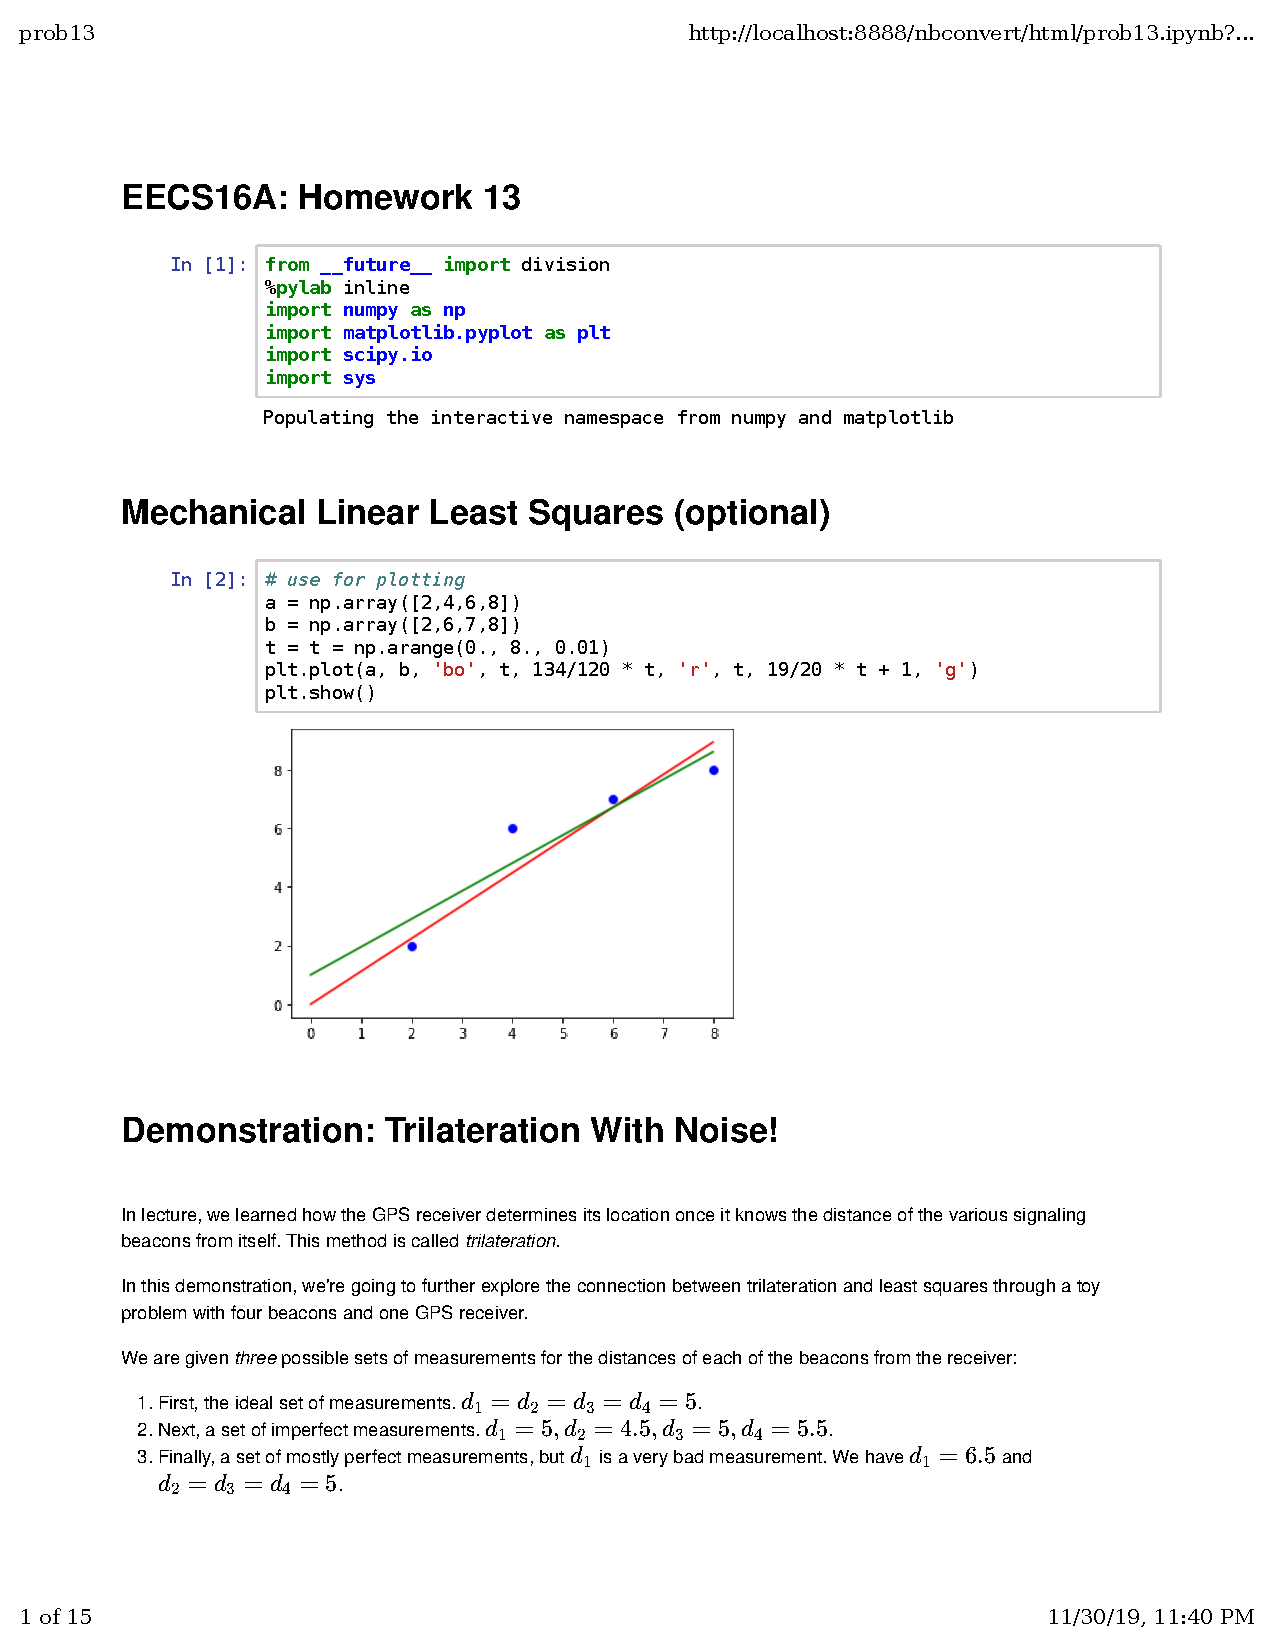
\includepdf[pages=-]{prob13.pdf}

\end{document}
